

%%%%%%%%%%%%%%%%%%%%%%%%%%%%%%%%%%%

\begin{frame}
\frametitle{Filtros Combados}

\vspace{-0.2cm}

\begin{itemize}
\footnotesize
\item Son filtros con múltiples bandas de paso y de supresión que tienen una respuesta en frecuencia que es una función periódica en w con periodo $\frac{2\pi}{L}$.
\visible<2->{

\item Se pueden generar a partir de otros filtros discretos G(z) ya diseñados haciendo la transformación $H(z)=G(z^{L})$

\vspace{0.1cm}

$G(z)=\sum_{n=-\infty}^\infty g(n)z^{-n}$

\vspace{0.1cm}

$H(z)=G(z^L)=\sum_{n=-\infty}^\infty g(n)z^{-Ln}$

\vspace{0.1cm}

$H(e^{jw})=\sum_{n=-\infty}^\infty g(n)e^{-jLnw}=G(e^{jwL})$

\item Tenemos una compresión en frecuencia de las características del filtro $G(e^{jw})$. Como la transformada de Fourier en tiempo discreto es periódica en w, la compresión hace que se repita el comportamiento cada $2\pi/L$.

\item Diseño con Matlab de IIR combados:

\begin{itemize}

\item \color{blue}\texttt{[num,den]=iircomb(L,Bw,tipo);}\color{black}

\item Bw: ancho de banda de la comba (normalizado)
\item Tipo: 'peak', 'notch'
\end{itemize}
}





\end{itemize}
\end{frame}


\begin{frame}
\frametitle{Ejemplos de FIR Combados}
\footnotesize

\color{olivegreen} Estudiar la respuesta en frecuencia que se obtiene al combar los siguientes filtros FIR:





\begin{columns}[c]
\begin{column}{4.5cm}

\vspace{0.5cm}


$G_1(z)=\frac{1}{2}(1+z^{-1})$

\vspace{0.2cm}

$G_2(z)=\frac{1}{3}(1+z^{-1}+z^{-2})$

\vspace{1.3cm}




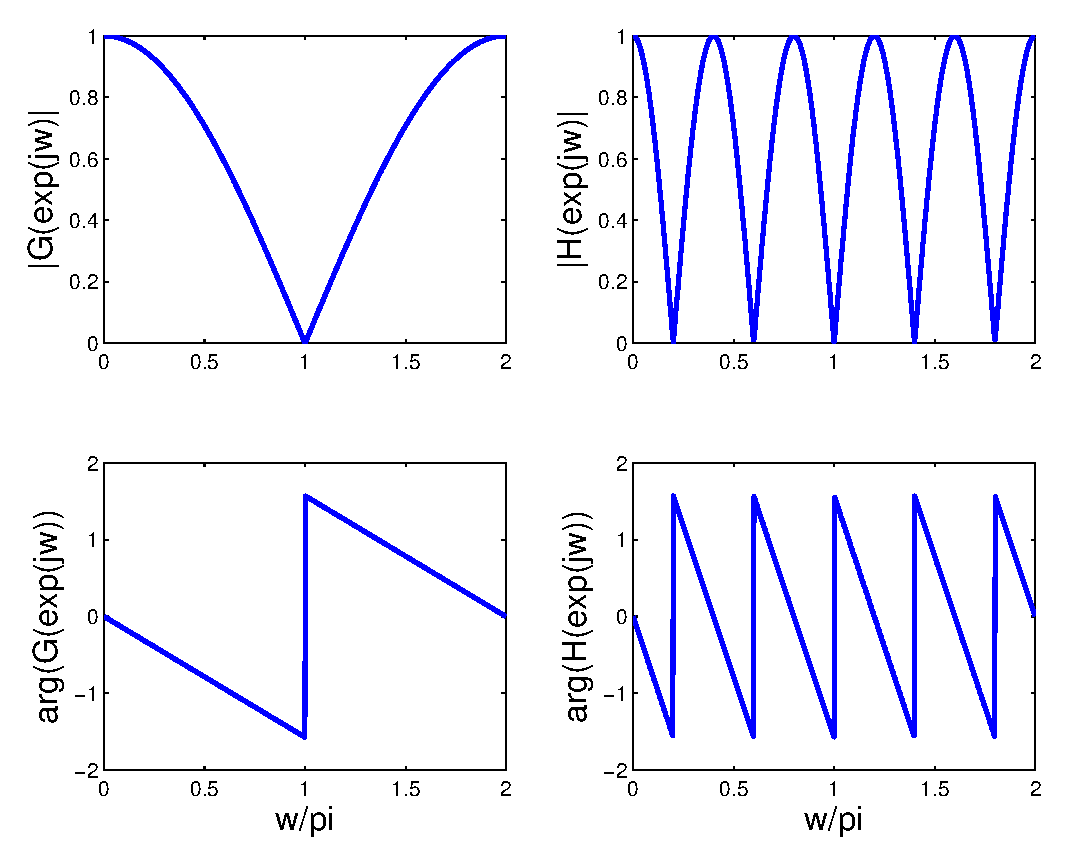
\includegraphics[width=4cm]{./Figures/EjCombFir2.eps}

\color{gray}

\hspace{1.5cm}$G_1(z)$

\end{column}
\begin{column}{5cm}

\color{gray}

\lstinputlisting{./Matlab/EjCombFIR.m}




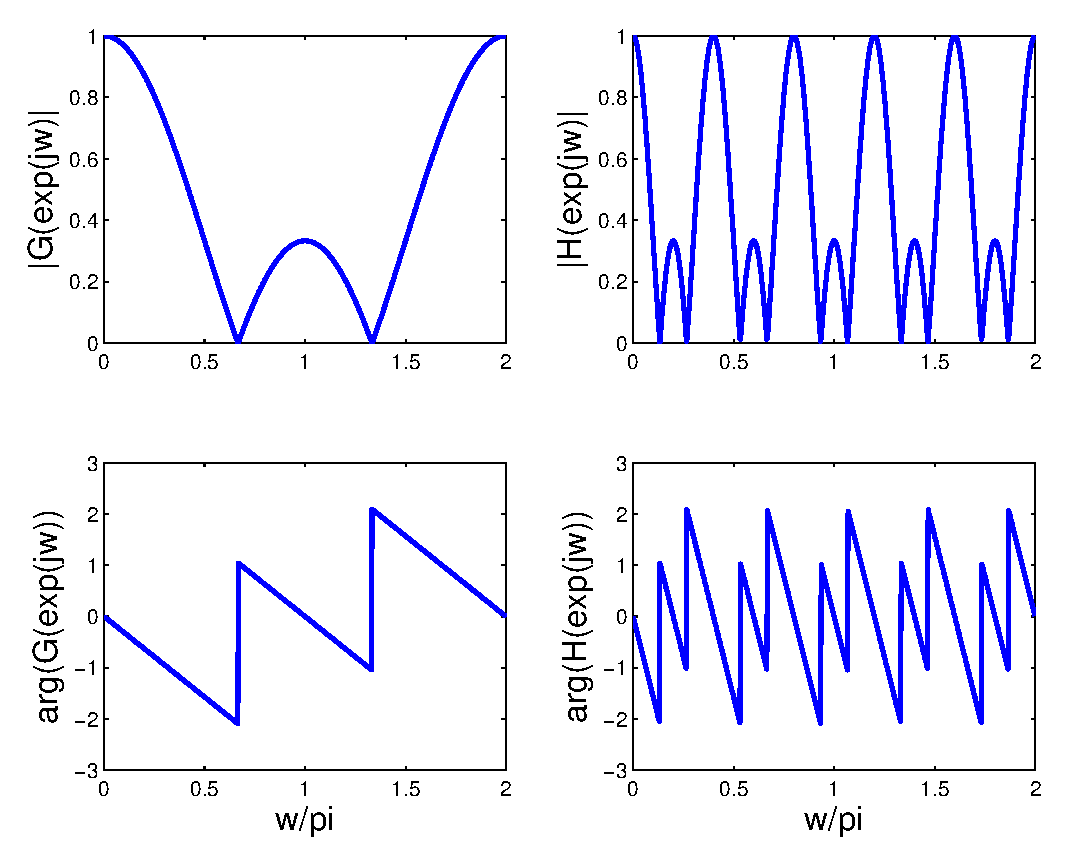
\includegraphics[width=4cm]{./Figures/EjCombFir3.eps}



\hspace{1.5cm}$G_2(z)$

\end{column}
\end{columns}


\end{frame}


%%%%%%%%%%%%%%%%%%%%%%%%%%%%%%%%%%%%%%%%


\begin{frame}
\frametitle{Ejemplos de IIR Combados}
\footnotesize

\color{olivegreen} Estudiar la respuesta en frecuencia que se obtiene al combar el siguiente filtro IIR:





\begin{columns}[c]
\begin{column}{4.5cm}

\vspace{0.5cm}


$G(z)=0.4\frac{1-z^{-1}}{1+0.2z^{-1}}$

\color{gray}

\lstinputlisting{./Matlab/EjCombIIR.m}



\end{column}
\begin{column}{5cm}

\color{gray}



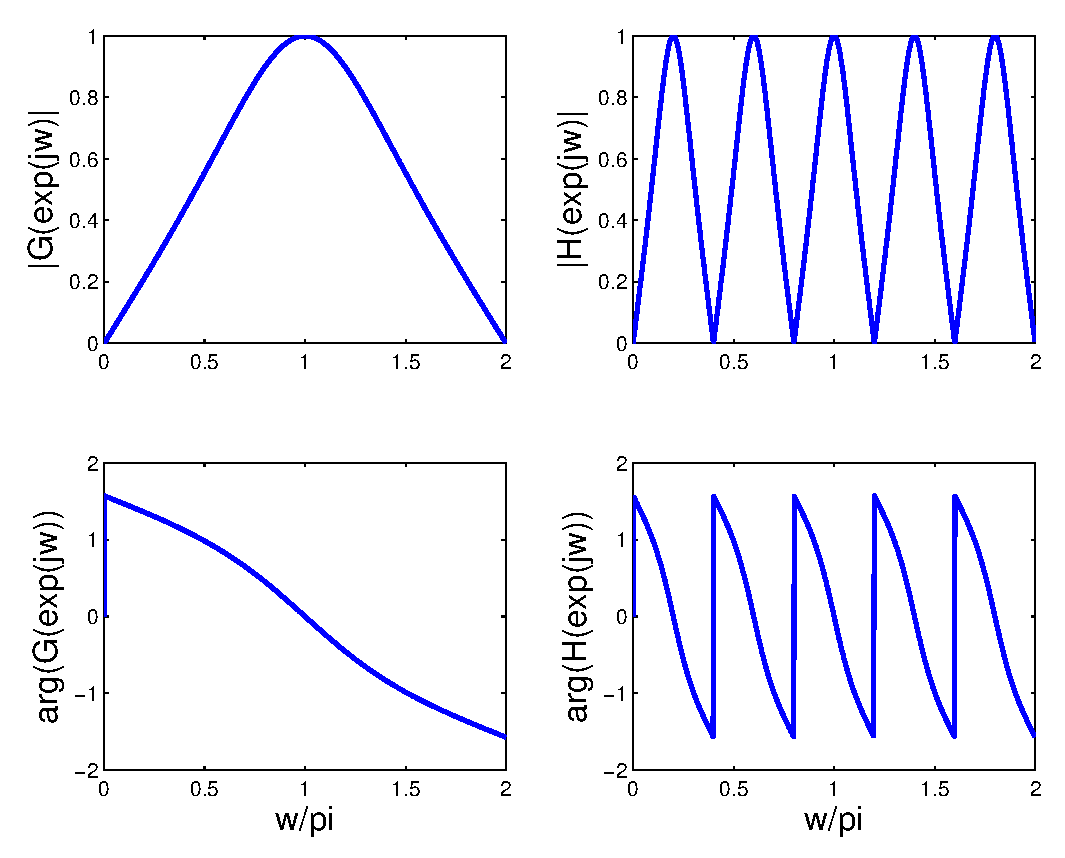
\includegraphics[width=4cm]{./Figures/EjCombIIR.eps}



\end{column}
\end{columns}


\end{frame}


%%%%%%%%%%%%%%%%


\begin{frame}
\frametitle{Ejemplos de IIR Combados con Matlab}
\footnotesize

\color{olivegreen} Diseñar un filtro combado para eliminar la f=15Hz y sus múltiplos para un sistema muestreo a f=300Hz.


\begin{columns}[c]
\begin{column}{4.5cm}

\vspace{0.5cm}

\color{gray}

$w_d=w_cT_s=2\pi \frac{f_{eliminar}}{f_s}=\frac{2\pi}{L}  \rightarrow L=\frac{f_s}{f_{eliminar}}=20$

$B_{w,max}=\frac{2\pi}{L}=0.314$

\lstinputlisting{./Matlab/EjCombIIRMatlab.m}



\end{column}
\begin{column}{5cm}

\color{gray}



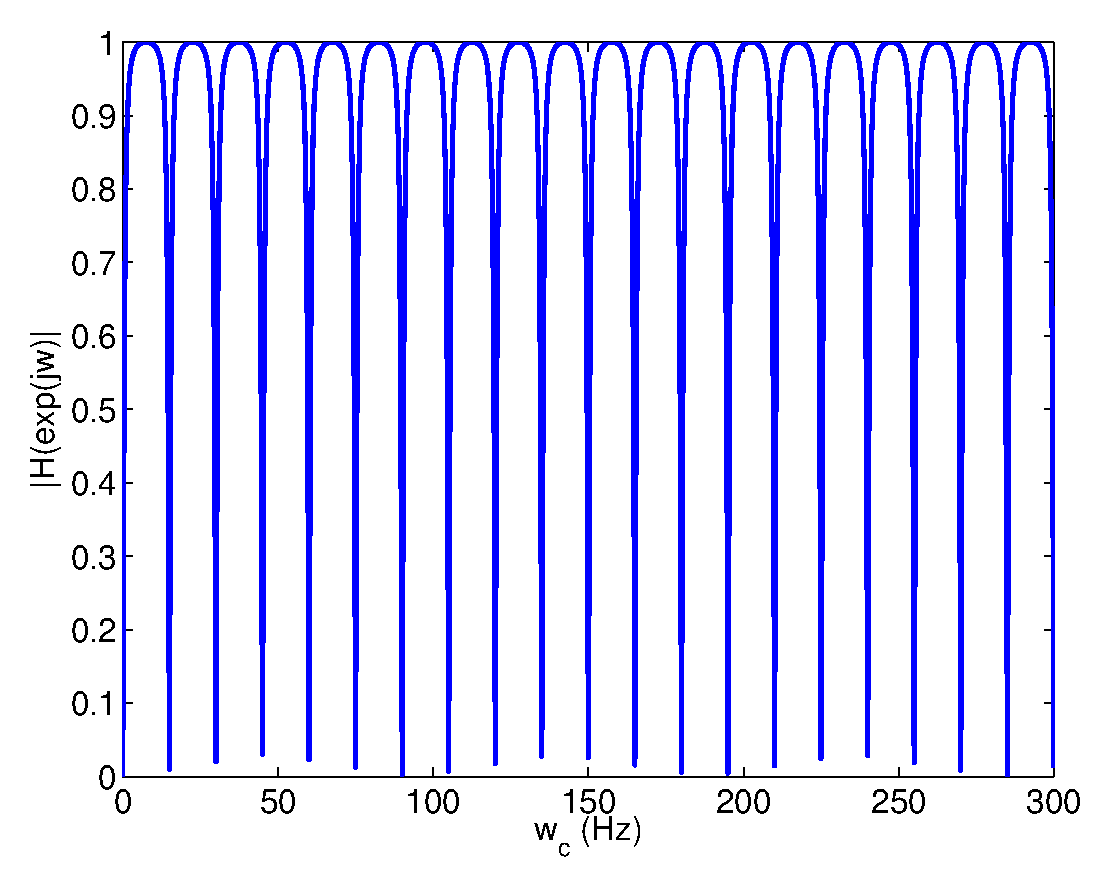
\includegraphics[width=4cm]{./Figures/EjCombIIRMatlab.eps}



\end{column}
\end{columns}


\end{frame}
